\section{Einführung in die Programmierung grafischer Benutezroberflächen mit JavaFX}


Eine grafische Benutzeroberfläche besteht i.d.R aus \textbf{Controls} und \textbf{Widgets}: \textbf{Buttons}, \textbf{Labels}, \textbf{Input-Elemente} (Textfelder)...\\

\noindent
Anordnung dieser Elemente wird mit Hilfe von Layouts realisiert, die verschachtelt sein können.\\

\noindent
Strukturen dieser Anordnungen können als Baumstrukturen verstanden werden, mit dem ``Fenster`` als Wurzel.\\

\noindent
In JavaFX wird ein Fenster als \code{Stage} bezeichnet.\\

\noindent
Das erste Fenster einer ANwendung muss man nicht selbst erstellen, sondern existiert bereits und wird zur Verfügung gestellt.\\

\noindent
Eine \code{Stage} beinhaltet keine UI Controls, sondern eine \code{Scene}, der dann weitere Elemente (i.d.R. zunächst ein ``Container``) hinzugefügt werden.\\

\noindent
Üblicherweise erzeugt man eine JavaFX-Anwendung, indem man von \code{javafx.application.Application} erbt, die \code{start()}-Methode überschreibt und darin die der Methode übergebenen \code{Stage} eine \code{Scene} zuweist und dann mittels \code{show()} sichtbar macht:

\begin{minted}[mathescape,
    linenos,
    numbersep=5pt,
    gobble=2,
    frame=lines,
    framesep=2mm]{java}
    public class JavaFxDemo extends Application {

        public void start(Stage primaryStage) {
            Hbox root = new Hbox();
            hbox.getChildren().add(...);
            ...
            Scene s = new Scene(hbox);
            ...
            primaryStage.setScene(scene);
            primaryStage.show();
        }

        public static void main(String[] args) {
            launch(args);
        }

    }
\end{minted}\\

\begin{tcolorbox}
    Die Methode \code{launch} ist blockierend, aus ihr kehrt man erst zurück, wenn die \textbf{PrimaryStage} geschlossen wurde.
\end{tcolorbox}

\noindent
Elemente werden Containern nicht mittels ``add`` o.ä. hinzugefügt, sondern man ruft die Liste der Kindelemente über \code{getChildren()} ab und fügt dieser dann die Kindelemente hinzu.\\

\noindent
Gibt man bei der \code{Scene} keine Größenangabe an, versucht JavaFX, die Fenstergröße so anzupassen, dass die Scene dargestellt werden kann.

\subsection{Ereignisbehandlung}

Nutzeraktionen werden ``Ereignisse`` genannt; die Behandlung solcher Ereignisse über Programmcode wird \textbf{Ereignisbehandlung} geannnt.\\

\noindent
So kann zum Beispiel ein \code{javafx.scene.control.Button} auf Mausereignisse reagieren, indem man

\begin{minted}[mathescape,
    numbersep=5pt,
    gobble=2,
    frame=none,
    framesep=2mm]{java}
    setOnAction(EventHandler<ActionEvent> value)
\end{minted}

implementiert. \code{value} enthält dann die Ereignisinformationen.

\begin{tcolorbox}
    Bei dem Typ des Parameters für die \code{setOnAction}-Methode handelt es sich um das \textit{Functional Interface}
     \begin{center}
     \code{java.fx.event.EventHandler<T extends Event>}
     \end{center}
    mit der abstrakten Methode \code{handle(T event)}\footnote{
        Interface EventHandler<T extends Event>: \url{https://docs.oracle.com/javase/8/javafx/api/javafx/event/EventHandler.html#handle-T-} - abgerufen 28.01.2024
    }
\end{tcolorbox}

\noindent
\textbf{Ereignisbehandlungen} werden i.d.R. durch \textbf{Upcalls} ausgelöst: Die JavaFX-Bibliothek enthält die Logik zur Verarbeitung nativer Ereignisse und ruft den Code des Entwicklers auf, die wiederum über \textbf{Downcalls} Logik der Bibliothek nutzen kann.

\begin{figure}
    \centering
    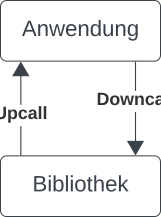
\includegraphics[scale=0.5]{chapters/fopt3/img/javafx/downcallupcall}
    \caption{Downcalls und Upcalls zwischen Anwendung und Bibliothek. (Quelle: eigene)}
    \label{fig:downcallupcall}
\end{figure}

\section{Properties, Bindings und JavaFX-Collections}

\subsection{Properties}

Das allgemeine Prinzip der Ereignisbehandlung basiert auf dem Entwurfsmuster \textbf{Observer}: $\rightarrow$ es gibt \textbf{beobachtbare Objekte} und \textbf{Beobachter}.\\

\noindent
\textbf{Beobachter} melden sich bei \code{beobachtbaren Objekten} an und werden über Zustandsänderungen benachrichtigt.\\

\noindent
Die Benachrichtigung erfolgt über Schnittstellenmethoden, die die Beobachter implementieren; die Schnittstellen sind die Typen der Parameter, die ein beobachtbares Objekt bei der Registrierung eines Beobachters berücksichtigen - es können also nur solche Objekte als Beobachter angemeldet werden, deren Klasse die Schnittstelle implementiert.\\

\noindent
\textbf{Properties} in JavaFX sind Klassen, die dieses Prinzip implementieren, und sind im Allgemeinen \textbf{beobachtbare Objekte}, bspw.

\begin{itemize}
    \item \code{SimpleIntegerProperty}
    \item \code{SimpleBooleanProperty}
    \item \code{SimpleObjectProperty<T>}
    \item {...}
\end{itemize}


\noindent
Spezielle varianten der Properties sind die \code{ReadOnlyProperty}s - diese können von \code{ReadOnlyWrapper}n zur Verfügung gestellt machen, um beobachtbare Properties öffentlich zu machen, aber deren Zustandsänderung von Außen zu untersagen.

\begin{minted}[mathescape,
    linenos,
    numbersep=5pt,
    gobble=2,
    frame=lines,
    framesep=2mm]{java}]
    public class Foo {

        private ReadOnlyIntegerWrapper value;

        ...

        public ReadOnlyInteger value() {
            return value.getReadOnlyProperty();
        }

        public void setValue(int v) {
            value.set(v);
        }

    }
\end{minted}\\

\subsection{Bindings}

Properties können miteinander gekoppelt werden, um gegenseitige Zustandsänderungen zu bewirken.\\

\noindent
Die Kopplung (das \textbf{Binding}) kann \textbf{unidirektion} oder \textbf{bidirektional} erfolgen.\\

\noindent
Bei \textbf{unidirektionalem} Binding bewirkt die Änderung des Wertes einer Property die Änderung des Wetes der anderen Property, aber nur in eine Richtung.\\
Wird versucht, über die andere Richtung eine Wertzuweisung durchzuführen, wird eine Exception geworfen.\\
Eine JavaFX-Property kann über \code{right.bind(left)} gekoppelt werden (lies: ``binde right an left``).\\

\noindent
Ein \textbf{bidirektionales} Binding bewirkt die Änderung der Properties in beide Richtungen, allerdings muss hier die Methode \code{bindBidirectional} genutzt werden: \code{right.bindBidirectional(left)} (bzw. \code{left.bindBidirectional(right)}).


\begin{figure}
    \centering
    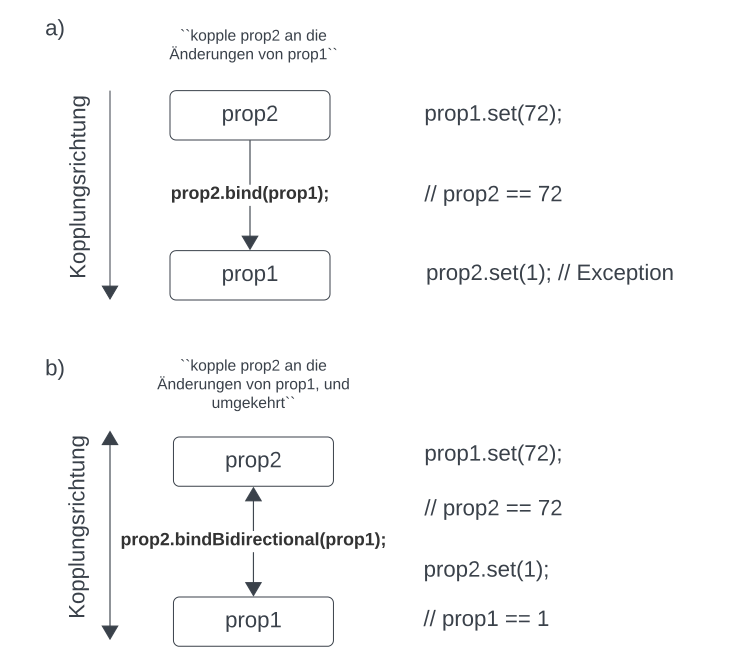
\includegraphics[scale=0.5]{chapters/fopt3/img/javafx/binding}
    \caption{Unidirektionales (a) und Bidirektionales (b) Binding in JavaFX. Die Properties sind vom Typ SimpleIntegerProperty. (Quelle: eigene)}
    \label{fig:binding}
\end{figure}